\documentclass{article}
\usepackage[utf8]{inputenc}
\usepackage{polski}
\usepackage{geometry}
\usepackage{pdfpages}
\usepackage{pdfpages}
\usepackage{listings}
\usepackage{listingsutf8}
\usepackage{multirow}
\usepackage{siunitx}
\usepackage{multirow}
\usepackage{booktabs}
\usepackage{tabularx}
\usepackage{placeins}
\usepackage{pdflscape}
\usepackage{graphicx}
\usepackage{subfig}
\usepackage{hyperref}
\usepackage{amsmath}

\geometry{
a4paper,
total={170mm,257mm},
left=20mm,
top=20mm
}
\newcolumntype{Y}{>{\centering\arraybackslash}X}
\renewcommand\thesection{}
\lstset{%
literate=%
 {ą}{{\k{a}}}1
 {ę}{{\k{e}}}1
 {Ą}{{\k{A}}}1
 {Ę}{{\k{E}}}1
 {ś}{{\'{s}}}1
 {Ś}{{\'{S}}}1
 {ź}{{\'{z}}}1
 {Ź}{{\'{Z}}}1
 {ń}{{\'{n}}}1
 {Ń}{{\'{N}}}1
 {ć}{{\'{c}}}1
 {Ć}{{\'{C}}}1
 {ó}{{\'{o}}}1
 {Ó}{{\'{O}}}1
 {ż}{{\.{z}}}1
 {Ż}{{\.{Z}}}1
 {ł}{{\l{}}}1
 {Ł}{{\l{}}}1
}

\title{Metody Obliczeniowe w Nauce i Technice\\ 
Laboratorium I}
\author{Maciej Trątnowiecki}
\date{AGH, Semestr Letni, 2020}

\begin{document}
    \maketitle
    \section{Sumowanie liczb pojedynczej precyzji}
        W ramach laboratorium zaimplementowałem trzy algorytmy obliczające sumę $N$ liczb z tablicy, każdej o wartości $v$. Za $N$ przyjąłem $10^7$, za $v$ początkowo $v=0.53125$. \\
        Obliczyłem błąd względny i bezwzględny jakim obarczone były przeprowadzone operacje arytmetyczne, uzyskując poniższe wyniki. 
        \begin{center}
            \begin{table}[ht]
                \centering
                \begin{tabular}{|c|c|c|c|}
                    \hline
                    Mierzona wartość & Sumowanie proste & Sumowanie rekursywne & Sumowanie Kahana\\
                    \specialrule{1pt}{1pt}{1pt}
                    Wynik sumowania &  5030840.50 & 5312500.00 & 5312500.00\\
                    \hline
                    Błąd bezwzględny & 281659.50 & 0.00 & 0.00\\
                    \hline
                    Błąd względny & 5.30\% & 0.00\% & 0.00\%\\
                    \hline 
                \end{tabular}
                \caption{Wyniki obliczeń dla $v=0.53125$}
                \label{tab:my_label}
            \end{table}
        \end{center}
        Następnie zmieniłem wartość $v$ na $0.63211$, uzyskując poniższe wyniki. 
        \begin{center}
            \begin{table}[ht]
                \centering
                \begin{tabular}{|c|c|c|c|}
                    \hline
                    Mierzona wartość & Sumowanie proste & Sumowanie rekursywne & Sumowanie Kahana\\
                    \specialrule{1pt}{1pt}{1pt}
                    Wynik sumowania &  6119759.50 & 6321100.00 & 6321100.00\\
                    \hline
                    Błąd bezwzględny & 201340.50 & 0.00 & 0.00\\
                    \hline
                    Błąd względny & 3.18\% & 0.00\% & 0.00\%\\
                    \hline 
                \end{tabular}
                \caption{Wyniki obliczeń dla $v=0.63211$}
                \label{tab:my_label}
            \end{table}
        \end{center}
        Błąd względny w algorytmie prostym znacznie rośnie, ponieważ wielokrotnie sumuje on liczby zupełnie różnych rzędów wielkości. Błąd względny jest znacznie mniejszy w algorytmie Kahana, jak i sumowania rekursywnego względem algorytmu prostego. W algorytmie rekursywnym, błąd nie występuje, ponieważ sumowane liczby są tego samego rzędu. Algorytm Kahana śledzi występujący błąd obliczeń i minimalizuje go w kolejnych sumowaniach.\\ %TODO: Co robi err? 
        Prześledziłem również jak wyglądał wzrost błędu w algorytmie prostego sumowania. Zebrane wyniki przedstawiłem na poniższych wykresach. Błękitnymi kropkami oznaczono każdy milion kroków. 
        \begin{figure}[h!]
            \centering
            \subfloat[$v=0.53125$]{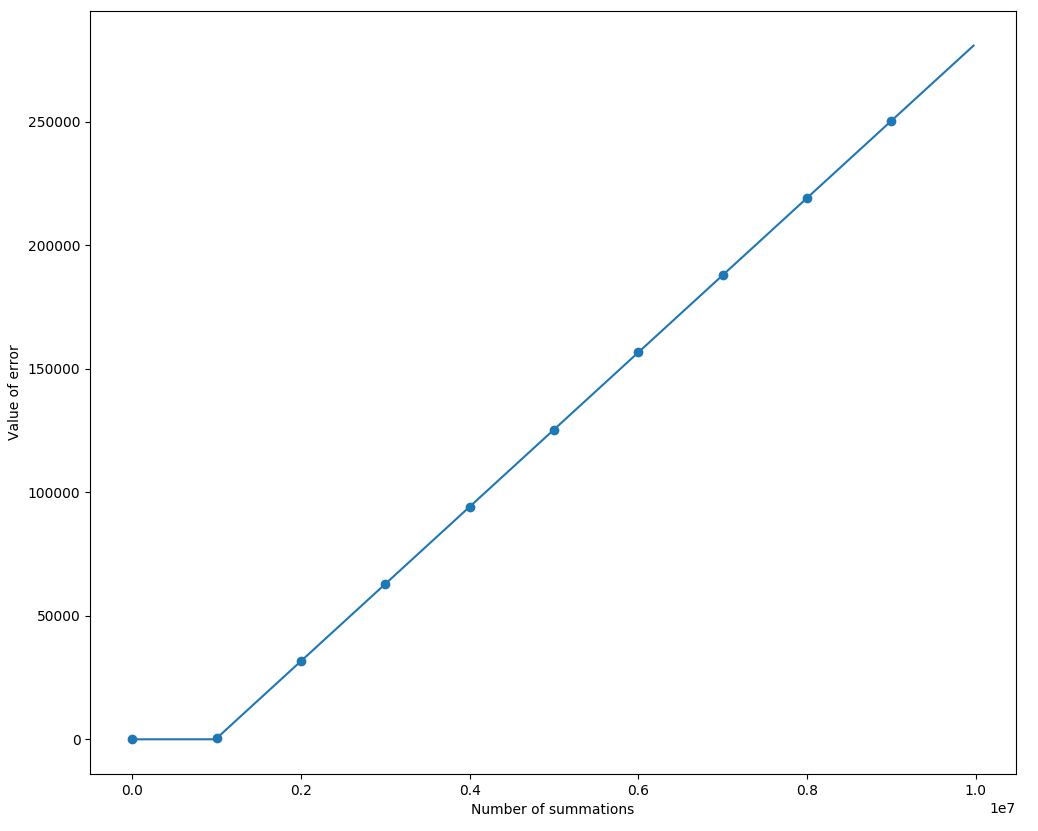
\includegraphics[width=9cm]{lab1/img/ErrorsPlot_1.png}}
            \subfloat[$v=0.63211$]{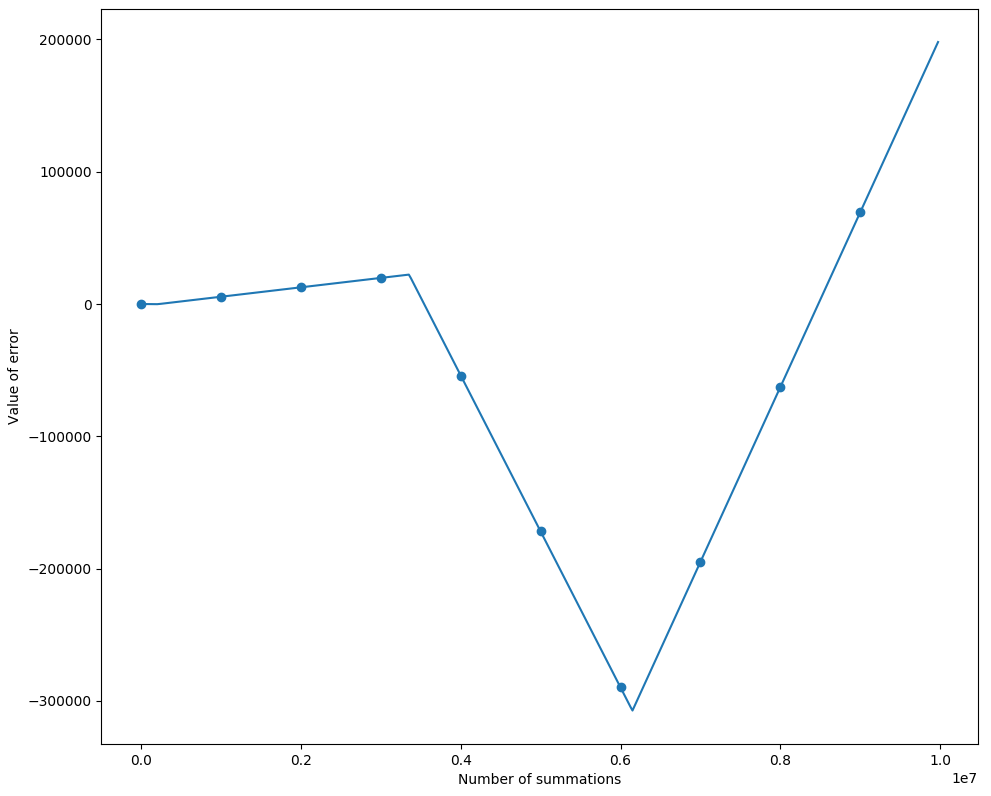
\includegraphics[width=9cm]{lab1/img/ErrorsPlot_2.png}}
            \caption{Wykres zmiany błędu bezwzględnego w stosunku do liczby sumowań.}
        \end{figure}\\
        Łatwo zauważyć, że wykres narastania błędu jest ciągłą sumą funkcji liniowych. W początkowej fazie, gdy dodawane wartości są tego samego rzędu, błąd nie rośnie w ogóle, lub rośnie wolno. 
        \FloatBarrier
        Wykonałem także porównanie czasów wykonania dla każdego z trzech algorytmów. Do pomiarów czasu w sposób powtarzalny użyłem pakietu sio2jail (\url{https://github.com/sio2project/sio2jail}), którego specyfika została lepiej opisana w pracy licencjackiej (\url{https://hitagi.dasie.mimuw.edu.pl/files/licencjat/pracalic-logo.pdf}), za pośrednictwem skryptu opakowującego oiejq (\url{https://oi.edu.pl/static/attachment/20181007/oiejq.tar.gz}), używanego przez Ogólnopolską Olimpiadę Informatyczną. Otrzymałem następujące wyniki.\\
        \begin{center}
            \begin{table}[ht]
                \centering
                \begin{tabular}{|c|c|}
                    \hline
                    Algorytm  & Czas wykonania \\
                    \specialrule{1pt}{1pt}{1pt}
                    Prosty & $21ms$ \\
                    \hline
                    Rekursywny & $156ms$ \\
                    \hline
                    Kahana & $21ms$ \\
                    \hline 
                \end{tabular}
                \caption{Pomiar czasów wykonania}
                \label{tab:my_label}
            \end{table}
        \end{center}\\
        Dla uprzednio rozważanych wartości $v$ zarówno algorytm rekursywny, jak i algorytm Kahana zwracał dokładny wynik. Jednak dla $v=0.666666$ w wyniku działania algorytmu rekursywnego otrzymałem wynik obarczony błędem bezwzględnym rzędu $0.50$, podczas gdy algorytm Kahana zwrócił wynik dokładny. 
        
    \section{Błędy zaokrągleń i odwzorowanie logistyczne}
        W celu prześledzenia zbieżności procesu iteracyjnego określonego zadanym odwzorowaniem logistycznym przygotowałem interaktywny wykres wartości kolejnych elementów ciągu dla wartości stałej $r$ z przedziału $[1.0, 4.0]$ i $x_0 = 0.77$. Ze względu na ograniczenia techniczne formatu pdf, wspomniany wykres umieściłem pod poniższym adresem \url{http://users.v-lo.krakow.pl/~maciektr/mownit/lab1_logistic_map.gif}.\\
        Za jego pomocą łatwo wywnioskować, że:
        \begin{itemize}
            \item dla $r\in[1.0,2.0]$ - kolejne elementy ciągu szybko zbiegają do swojej granicy. Możemy prosto wyznaczyć ją sposobem wspomniany poniżej.
            \item dla $r\in[2.0,3.0]$ - ciąg jest zbieżny, ale w początkowej fazie waha się. 
            \item dla $r\in[3.0,3.5]$ - odwzorowanie tworzy oscylator.
            \item dla $r\in[3.5,4.0]$ - otrzymujemy chaotyczne drgania. 
        \end{itemize}
        Załóżmy, że ciąg $x_n$ jest zbieżny. Niech $\lim_{n\to\infty} x_n=g$. Wtedy: 
        $$\lim_{n\to\infty} x_{n+1}=g=\lim_{n\to\infty} rx_n(1-x_n)=rg(1-g)\implies r(1-g)=1 \implies g=\frac{r-1}{r}$$
        Następnie przygotowałem wykres bifurkacyjny dla zadanego odwzorowania. Oryginalny obraz, o rozdzielczości $4000x4000$ pikseli umieściłem pod następującym adresem \url{http://users.v-lo.krakow.pl/~maciektr/mownit/lab1_bifurcation.png}.
        \begin{figure}[h!]
            \centering
            \subfloat[$x_0=0.7;r\in(1.0, 4.0)$]{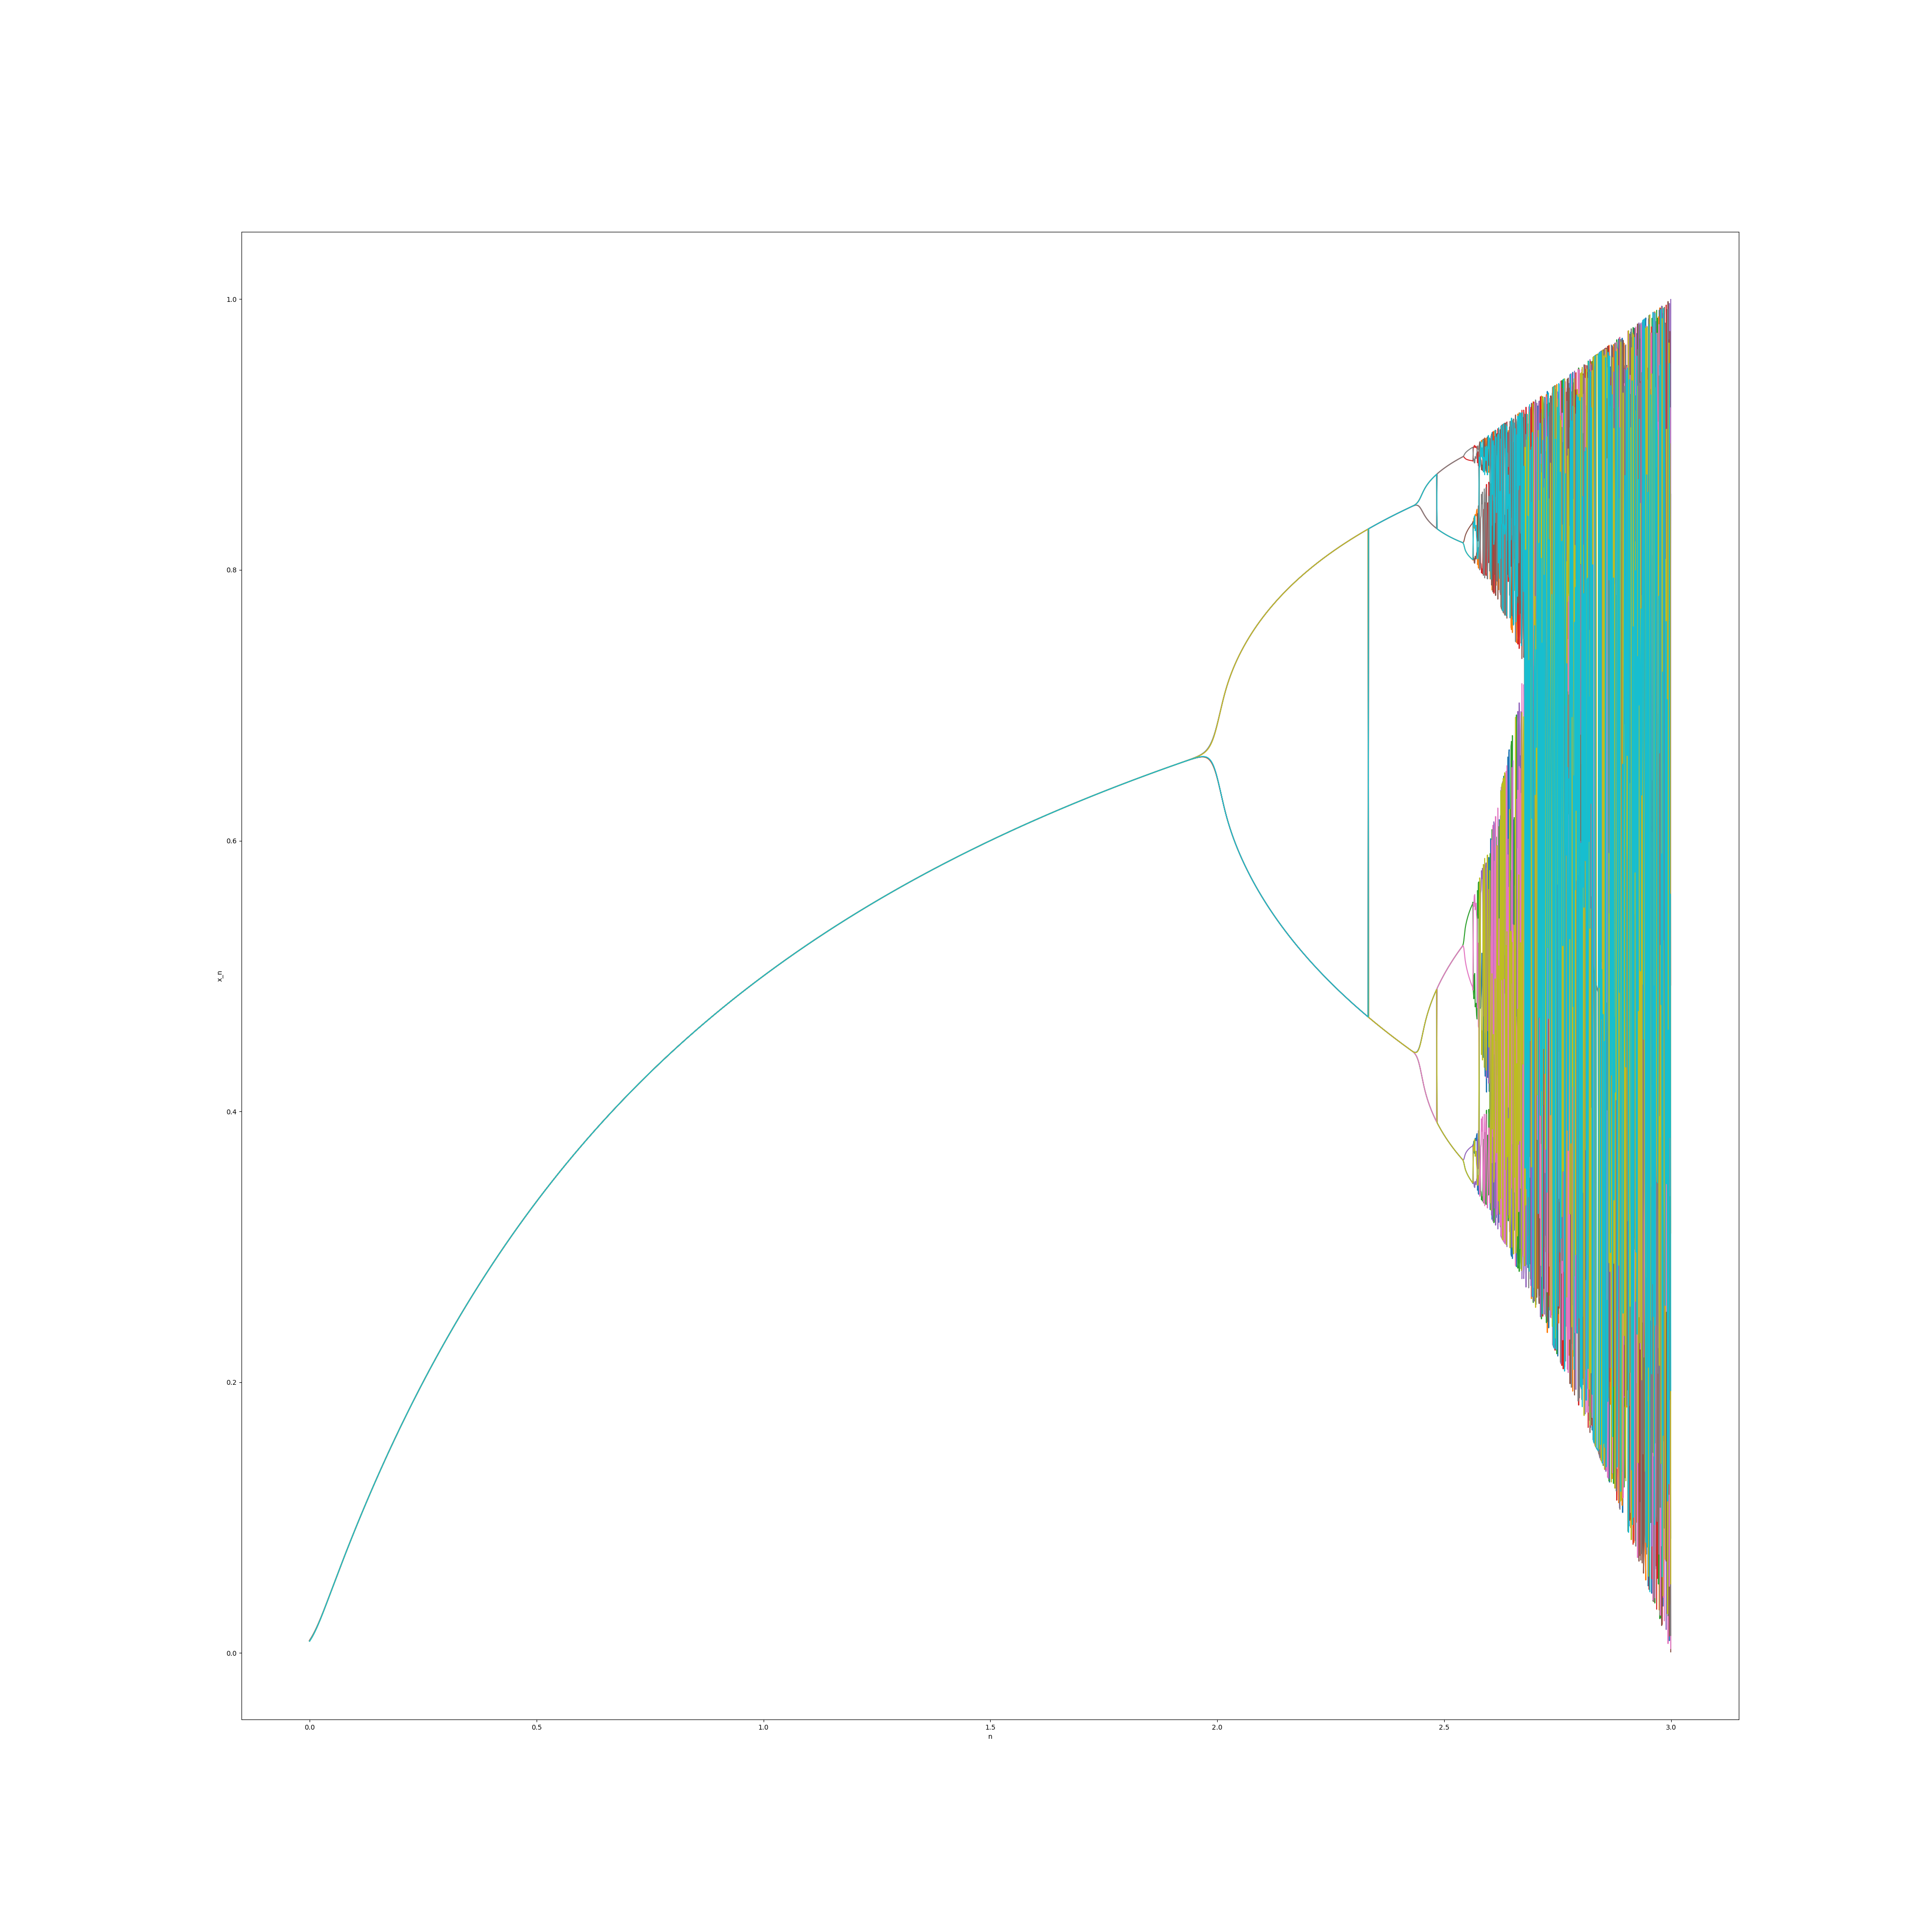
\includegraphics[width=18cm]{lab1/img/Bifurcation_0.png}}
            \caption{Diagram bifurkacyjny.}
        \end{figure}
        \begin{figure}[h!]
            \centering
            \subfloat[$x_0=0.7;r\in(3.5, 4.0)$]{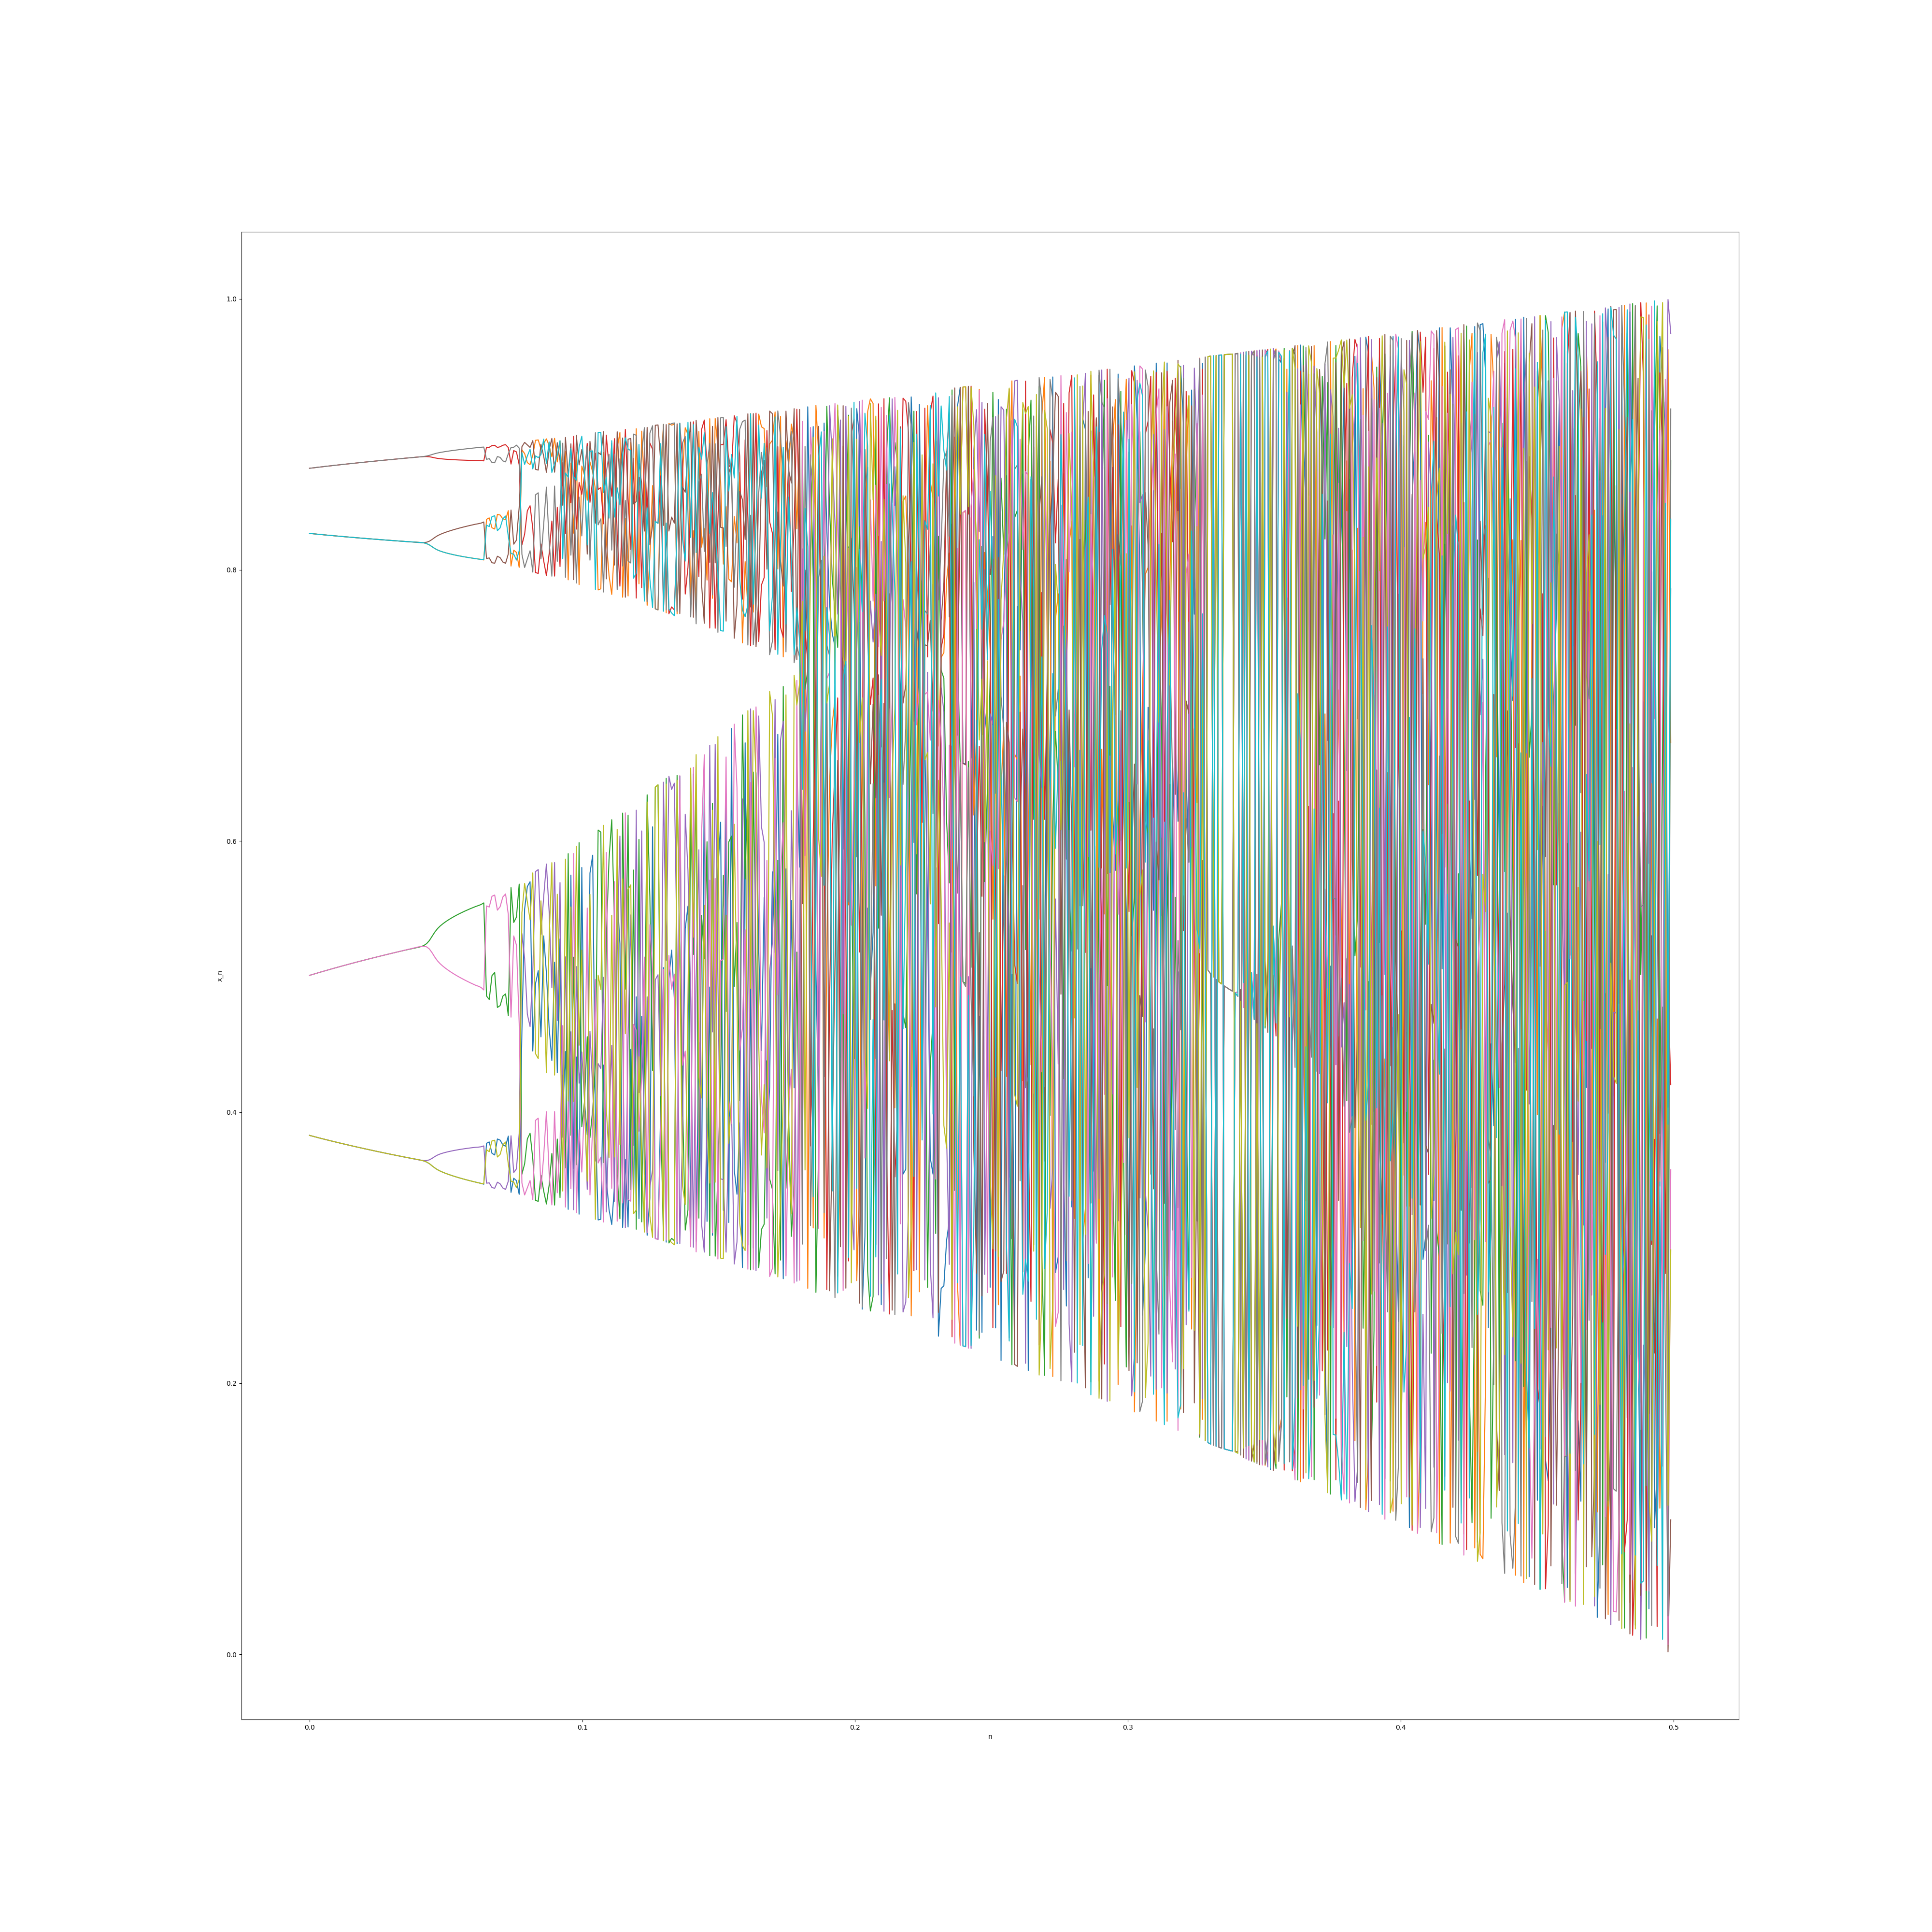
\includegraphics[width=13cm]{lab1/img/Bifurcation_3.png}}\\
            \subfloat[$x_0=0.8;r\in(1.0, 4.0)$]{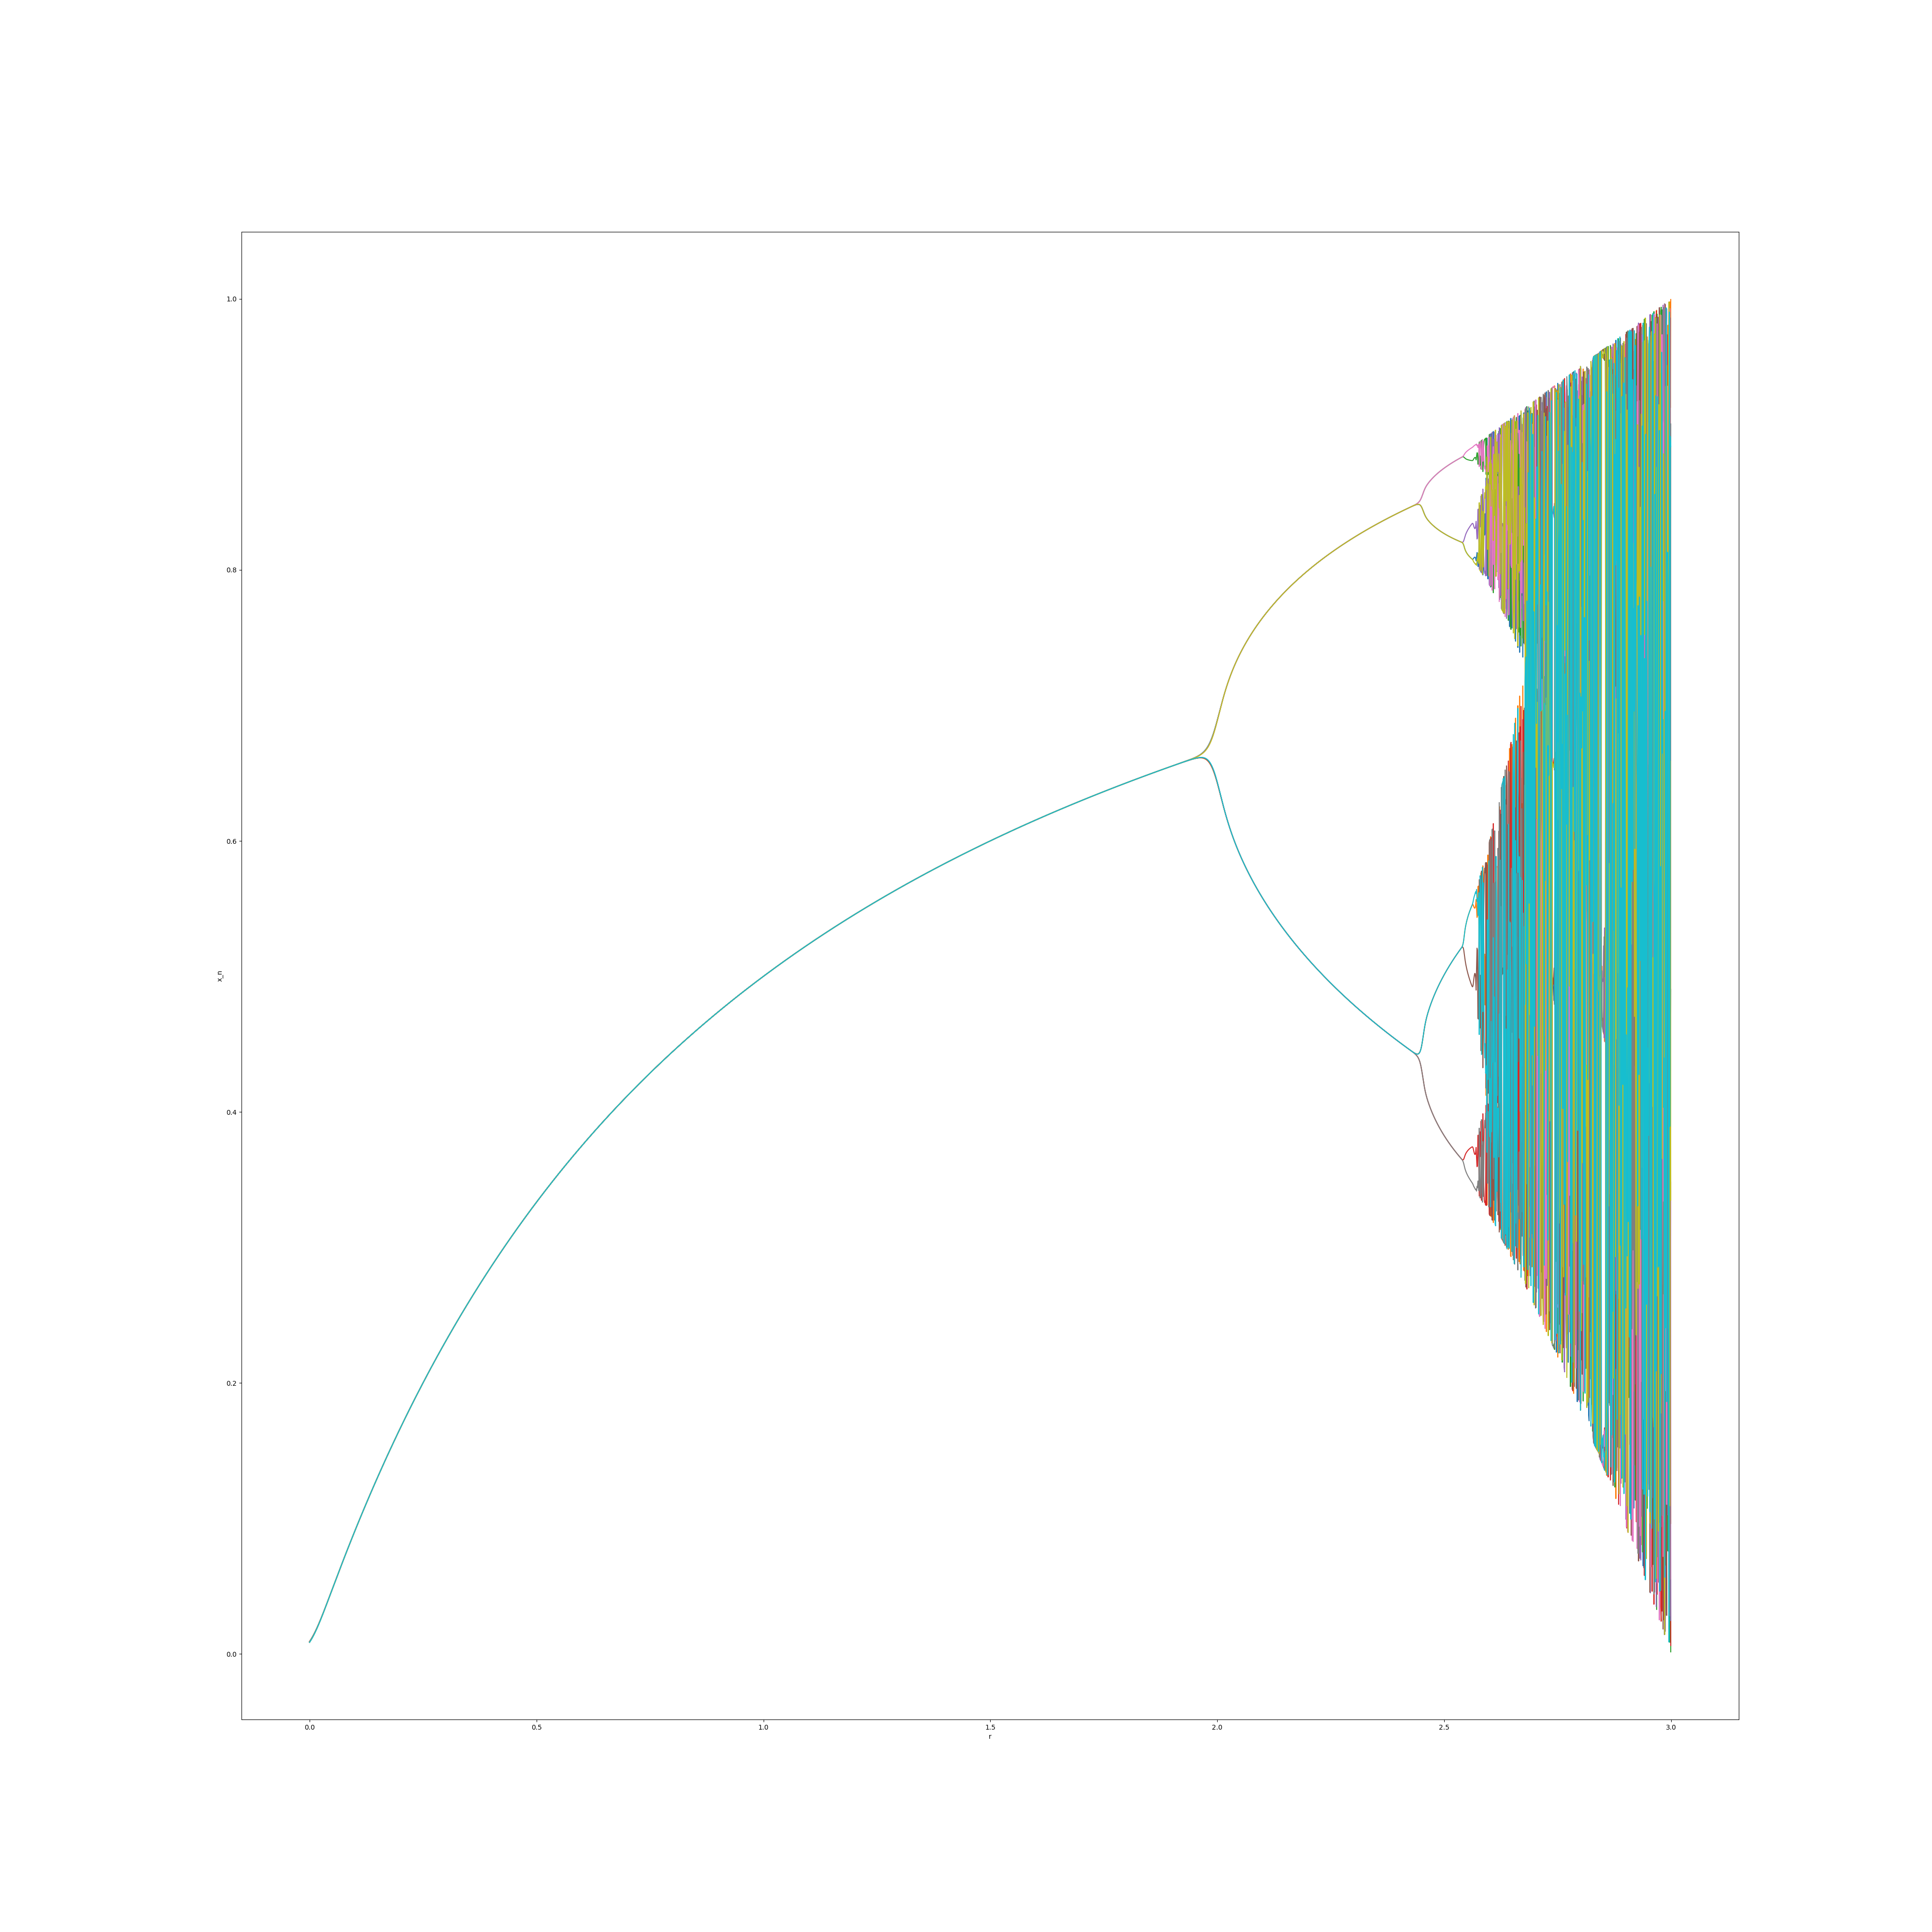
\includegraphics[width=13cm]{lab1/img/Bifurcation_6.png}}
            \caption{Diagram bifurkacyjny.}
        \end{figure}\\
        Diagram bifurkacyjny pokazuje rozwidlanie się stanów stabilnych odwzorowania logistycznego. Łatwo zauważyć związek otrzymanego wykresu, z wcześniej określonymi przedziałami zbieżności. 
        \FloatBarrier
        Prześledziłem również zmianę trajektorii liczonych z użyciem pojedynczej i podwójnej precyzji. 
        \begin{figure}[h!]
            \centering
            \subfloat[$x_0=0.7;r\in(3.5, 4.0)$]{\includegraphics[width=13cm]{lab1/img/Tra1}}\\
            \subfloat[$x_0=0.8;r\in(1.0, 4.0)$]{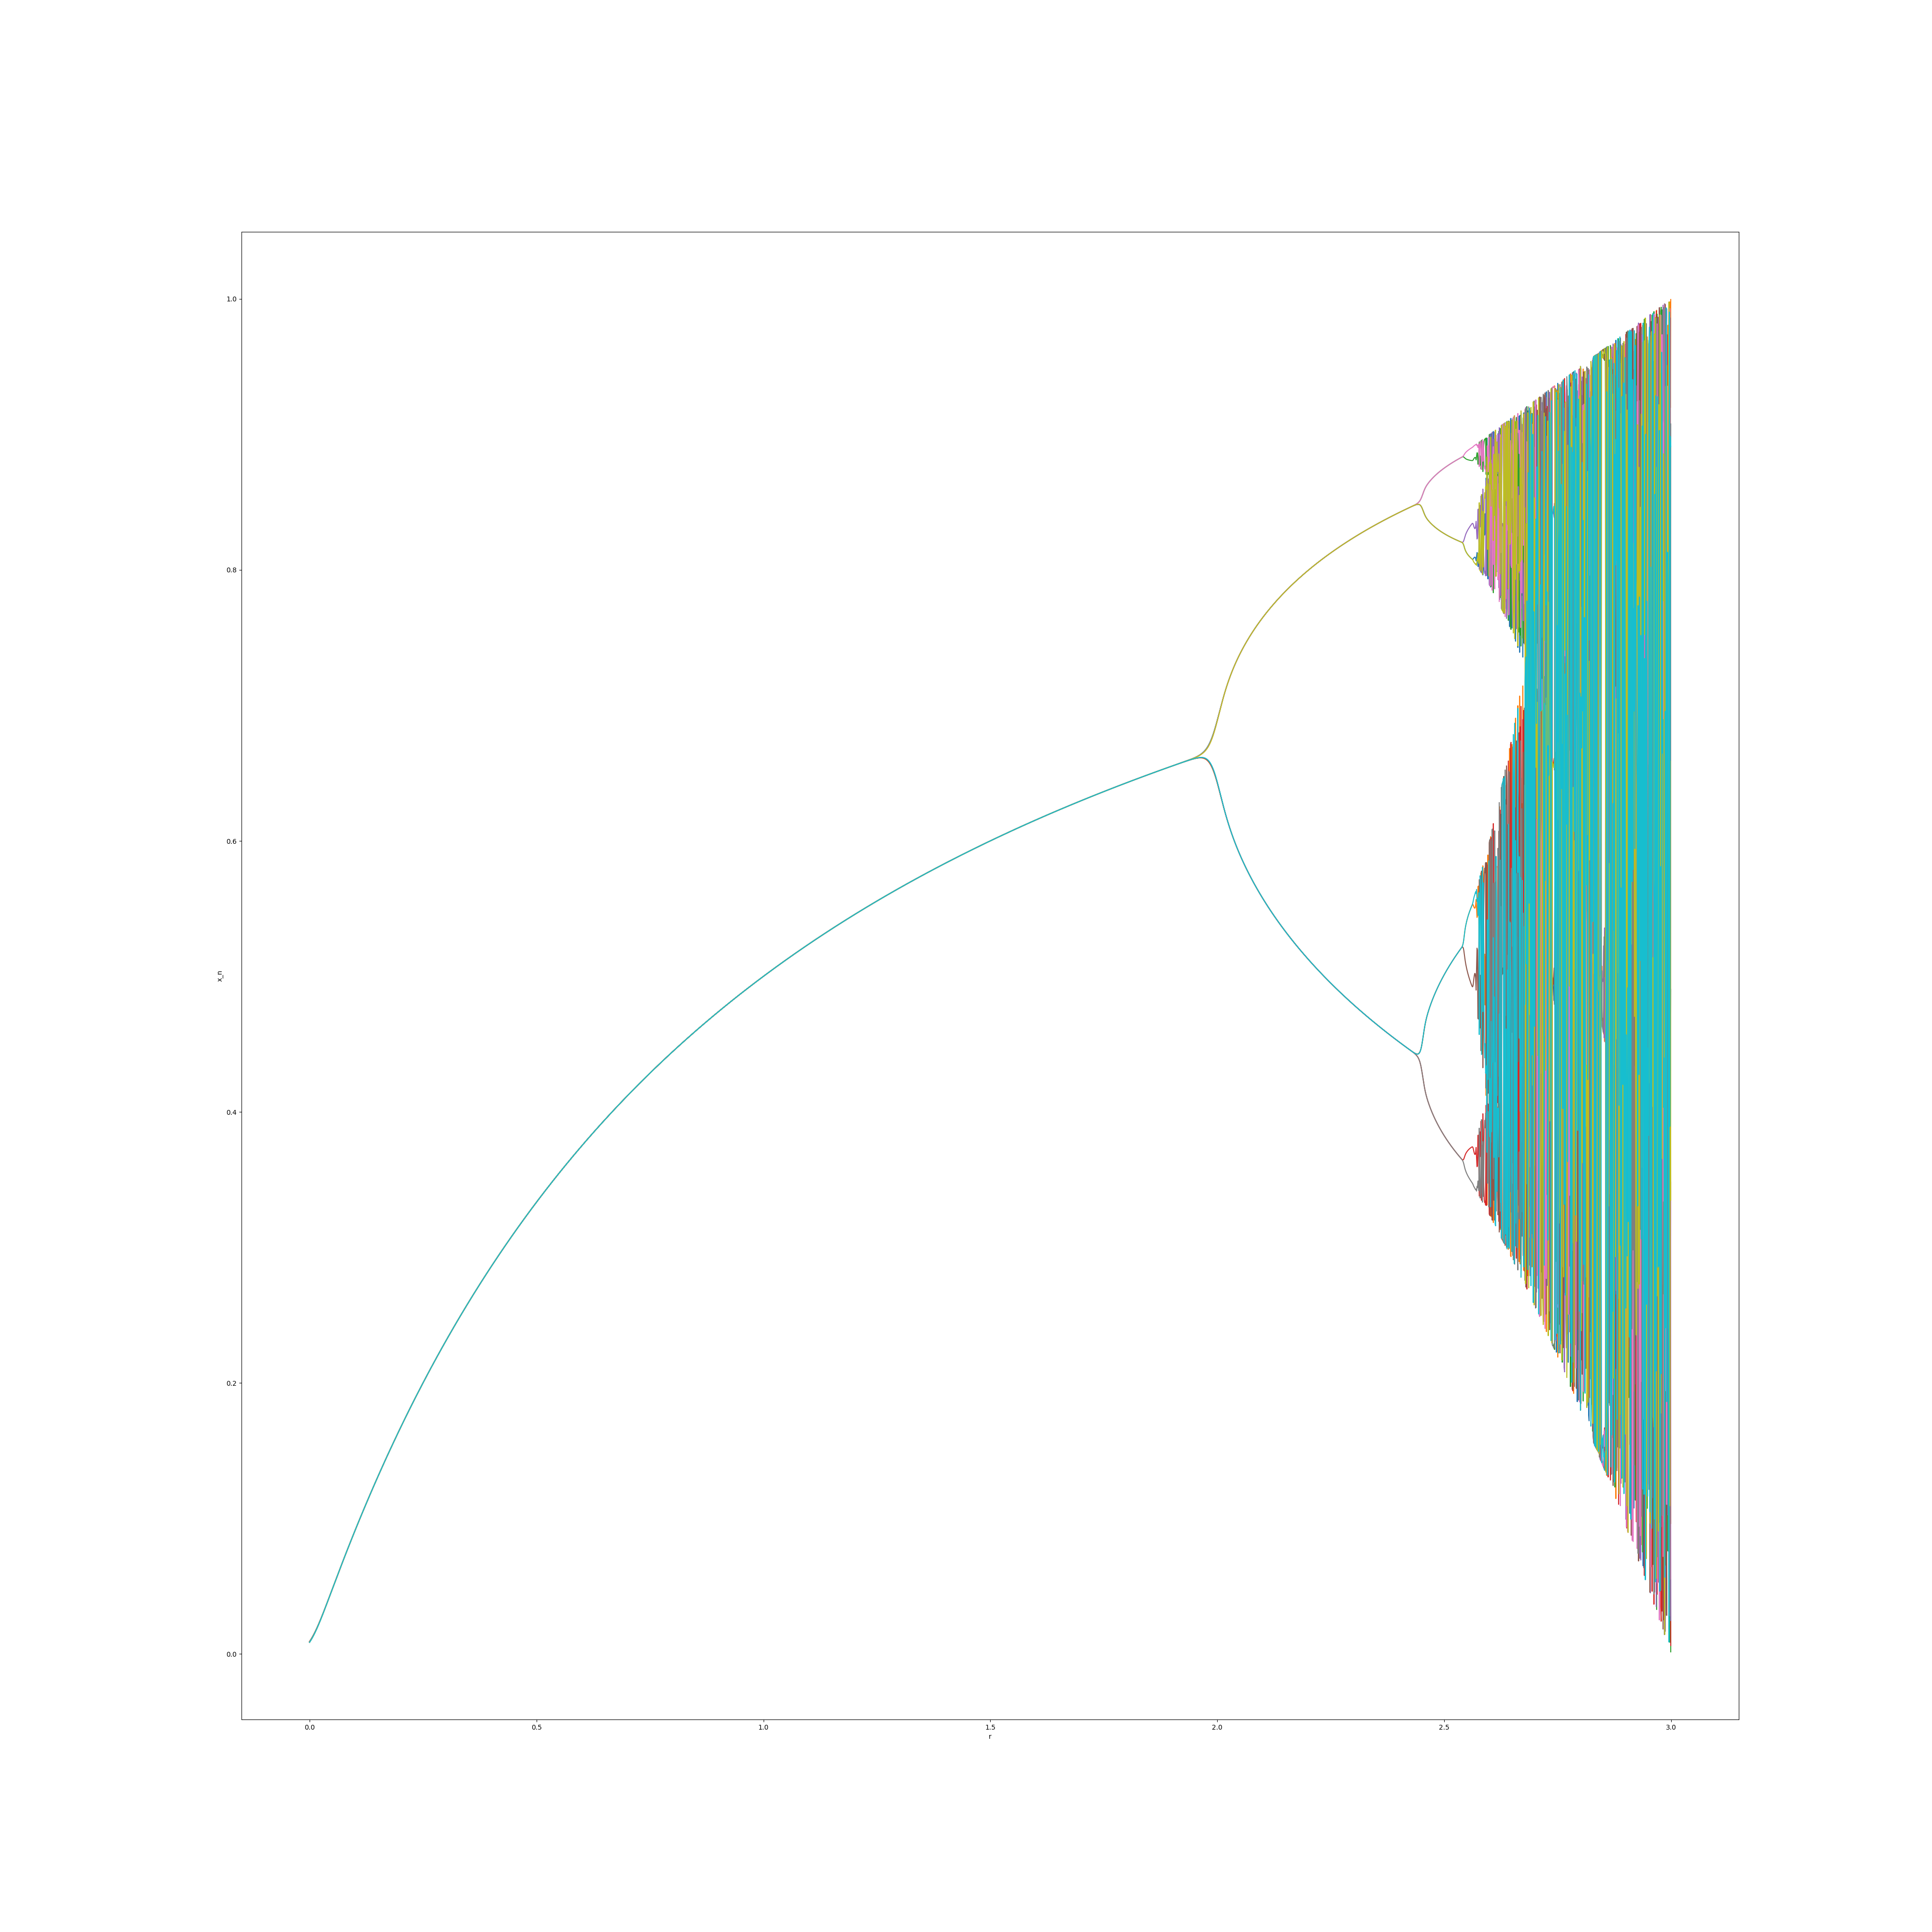
\includegraphics[width=13cm]{lab1/img/Bifurcation_6.png}}
            \caption{Diagram bifurkacyjny.}
        \end{figure}\\
        

        
    
\end{document}